\documentclass[a4paper,11pt,titlepage,uplatex]{jsreport}

\usepackage{etoolbox}
\makeatletter
\patchcmd{\chapter}{\if@openleft\cleardoublepage\else\if@openright\cleardoublepage\else\clearpage\fi\fi}{}{}{}
\makeatother

\setcounter{tocdepth}{3}

% \usepackage{titlesec}
% \titleformat*{\chapter}{\large\bfseries}

% 数式
\usepackage{amsmath,amsfonts}
\usepackage{bm}
% 画像
\usepackage[dvipdfmx]{graphicx}
\usepackage{here}

\usepackage[hang,small,bf]{caption}
\usepackage[subrefformat=parens]{subcaption}
\captionsetup{compatibility=false}


\begin{document}

\begin{titlepage}
  \noindent
  \begin{flushright}
    \underline{令和4年度 \space 卒業論文}
  \end{flushright}
  \vspace{3cm}
  \begin{center}
    \fontsize{20pt}{1cm}\selectfont
    炉物理パラメータ不確かさ評価における

    複数の模擬パラメータを活用した
    
    無次元化CV-S法

    \vspace{3cm}

    \fontsize{18pt}{2cm}\selectfont
    原子炉工学研究室

    鷹見大地

    \vspace{6cm}

    \fontsize{10pt}{0cm}\selectfont
    北海道大学 工学部 機械知能工学科
    \end{center}
    
\end{titlepage}


\tableofcontents
\clearpage

\chapter{序論}
\section{背景}
\subsection{炉物理計算結果の不確かさ}
工学の分野において、数値計算によってシステムの特性値、パラメータを予測することが一般的に行われている。
計算モデルや計算手法、アルゴリズムの高度化によって数値計算の予測値の精度を向上させることは重要であるが、
それと同時に、予測値が内包する不確かさを定量化することも、計算結果の信頼性の向上や効率的な研究開発の実現などの観点から重要である。
原子炉工学の分野、特に原子炉物理の分野において、不確かさの定量化に関する研究が、この20年、活発に行われてきている。

原子炉物理分野において、数値計算の予測値の不確かさの要因はいくつかあるが、入力情報の1つとして用いられる
核データの不確かさが主なものの一つとして挙げられる。
それを受けて、核データの不確かさに起因する炉物理計算結果の不確かさの定量化が、核データ工学、原子炉物理を跨いだ重要な研究課題となっている。

核データの不確かさに起因する炉物理パラメータの不確かさを評価する方法は、感度係数を用いて誤差伝播を計算する方法\cite{cacucci1988forward}と
サンプリング法を用いる方法\cite{mckay1988sensitivity}とに大別される。前者は、感度係数を得るために摂動理論に基づく複雑な計算を行う必要があるが、
感度係数さえ得ることができれば計算時間を要さないという利点がある。ただし、感度係数は出力(炉物理パラメータ)の
入力(核データ)に対する一次微係数であることから、出力と入力に線形性が仮定されるため、厳密な誤差伝播計算を行うことができないという問題がある。
一方、後者は、前者の方法で導入される線形成の仮定が不要である一方で、膨大な計算時間を要するという短所がある。
また、サンプリング法で得られる結果(不確かさ)には必ず統計的な不確かさが含まれることになり、これを小さくするためには標本数を大きくとらなければいけない点にも留意する必要がある。

\subsection{制御変量法と感度係数}
これまでに、少ない標本数で不確かさの小さい結果を得るための効率的なサンプリング手法として、ラテン超方格法\cite{mckay1988sensitivity}や、決定論的サンプリング手法\cite{julier1997new}などが提案されてきた。
一方、我々の研究グループでは、感度係数を計算するためのコードを開発していることから、制御変量法(CV法)と呼ばれる方法と
感度係数を組み合わせて利用する方法(CV-S法)を考案し、核燃料の燃焼問題においてその有効性を示した\cite{nihira2019combination}。
CV法とは、評価対象とする出力パラメータ(対象パラメータ、ターゲットパラメータ)に対して、振る舞いが類似であり、
その統計量が既知、もしくは高精度な推定が容易な別なパラメータ(模擬パラメータ、モックアップパラメータ)を考え、
その2つのパラメータの差分に着目することで、少ない標本数で統計量を効率的に推定する方法である\cite{kroese2013handbook}。
これについての具体的な理論や計算手続きとしては、論文\cite{nihira2019combination}にまとめられたものが最初である。

CV-S法は、対象パラメータについて、入力に対して線形に振る舞う仮想的な出力パラメータを考え、これを類似パラメータと見做してCV法を適用する、というものである。
文献\cite{nihira2019combination}では、軽水炉の燃料ピンセルの燃焼問題に対して、この手法が適用された。また、CV-S法で類似パラメータとして扱われる、
入力に対して線形に振る舞う仮想的な出力パラメータは、必ずしも対象パラメータの線形近似である必要はない。
この点に着目し、燃料集合体の炉物理パラメータを対象パラメータとし、仮想的な模擬パラメータを、より簡易な燃料ピンセル体系の炉物理パラメータの一次近似とした検討を行い、
そのような場合であってもCV-S法が良好な性能を示すことが確認された\cite{kida2022enhancement}。

\subsection{CV法の高度化}
CV-S法では現在、以下で示す高度化が図られている。

CV法の原著論文(文献\cite{nihira2019combination})では、CV-S法の性能(不確かさの低減度合い)が対象パラメータと類似パラメータの平均値および標準偏差の違いに依存するという点が指摘されている。
直感的には、CV-S法の性能は、対象パラメータと類似パラメータの相関の強さのみに依存するものと考えられるが、文献\cite{nihira2019combination}のFigure 5、 6に示されているように、
対象パラメータと類似パラメータの平均値・標準偏差の違いにも影響されていることが分かっている。この問題点を解決するため、対象パラメータ、模擬パラメータの無次元化を行い、
無次元化されたパラメータに対してCV-S法を適用するという方法が提案され、簡易問題での検討を通してその妥当性が確かめられた\cite{suzuki2022}。

また、単一の模擬パラメータではなく、複数の模擬パラメータを合成した仮想的なパラメータを用いたCV-S法による性能向上も図られ、簡易問題と軽水炉燃料集合体の燃焼問題に対する適用性が評価された\cite{kida2022aki}\cite{kida2022syuusi}。
この複数の模擬パラメータの合成においては、拡張バイアス因子法で用いられている方法\cite{kugo2007theoretical}を使用するが、合成した擬似的な模擬パラメータの感度が対象パラメータの感度と極力類似となるように、
合成の際に用いる重みを決定する必要がある。既往研究では、遺伝的アルゴリズム(GA)の適用が試みられた\cite{kida2022aki}。

\section{研究目的}
CV-S法について、上述された方法がそれぞれ有効であることが確認された。しかし、いずれの検討も初歩的な段階にとどまっており、検証計算の充実や、複数の模擬パラメータを合成する際の重みの決定方法の吟味、高度化が必要とされている。
さらに、これら二つの手法を組み合わせることによりCV-S法の性能を向上させられる可能性もある。

このような背景から、本研究では、CV-S法におけるパラメータの無次元化と複数の模擬パラメータの合成の各々についてのより深い検討を実施すると共に、これらを併用したCV-S法を実現し、その性能を評価することを目的とする。
\newpage

\chapter{CV-S法による統計量の評価方法}
\section{不確かさ評価の流れ}
\subsection{概要}
以下の手順に従って不確かさ評価を行うプログラムを作成した。

\begin{enumerate}
  \item Box-Muller法を用いて正規分布に従う乱数を生成する。
  \item 1で得られた乱数を用いて入力パラメータをランダムサンプリングする。
  \item 入力パラメータから計算コードにより計算を行い、出力パラメータを得る。
  \item 得られた出力パラメータについて、不確かさ(標準誤差)の挙動を観察する。
\end{enumerate}

\subsection{従来の方法による評価対象とする統計の導出}
本研究では、以下の統計量を評価対象とする。

\begin{itemize}
  \item 期待値(平均値)… 確率変数はさまざまな値をとるが、それらの値を代表して、しばしば平均値が統計の実際的な局面で用いられる。一般に
  確率変数$X$に対して、それがとる値の重みつき平均を確率変数の期待値といい、$E\left[X\right]$と書く。また、$X$が連続型の確率分布を持つとき、$X$のとる値が関数$p\left(x\right)$によって
  \begin{equation}
    P\left( a \leq X \leq b \right) = \int_a^b p\left(x\right) dx 
    \label{eq2.1}
  \end{equation}
  と表される。この関数$p \left( x \right)$を$X$の確率密度関数という。このとき、確率変数$X$の期待値は式(\ref{eq2.2})で表される。
  \begin{equation}
    E\left[x\right] = \int_{-\infty}^{\infty} xp\left(x\right) dx 
    \label{eq2.2}
  \end{equation}

  \vspace{1.0\baselineskip}

  \item 分散 … 確率変数のばらつきを表す。期待値は確率変数の重要な指標の一つではあるが、あくまでその確率変数の一側面に過ぎず、期待値が同一でも確率変数が異なる場合も数多く存在する。
  そこでもう一つ重要な指標となるのが分散である。分散にもいくつかの種類が存在するが、ここでは不偏分散を用いる。これは、不偏分散が入力パラメータの真の値の推定に役立つからである。
  定義式は式(\ref{eq2.3})で表される。また、本研究における「不確かさ」とは、不偏分散の二乗根をとった標準偏差の値を指し、式(\ref{eq2.4})で定義される。
  \begin{equation}
    V\left[X\right] = E\left[ X^2 \right] - E\left[ X \right]^2
    \label{eq2.3}
  \end{equation}
  \begin{equation}
    \sigma \left[X\right] = \sqrt{V\left[ X\right]}
    \label{eq2.4}
  \end{equation}
\end{itemize}

\subsection{CV法による統計量の推定}
ここでは、統計量の推定を行う対象のパラメータ$X$と、それと振る舞いが類似で統計量が既知な模擬パラメータ$Y$を考える。

これらについて、一定の標本数セットを用意し、以下の手順に沿って対象のパラメータの期待値、分散およびそれらの標準誤差を求める。

\begin{itemize}
  \item 期待値$E\left[X\right]$
  
   まず、パラメータ$H_1 = X - \alpha Y$を用意する。これを用いることで、対象パラメータ$X$の期待値$E\left[X\right]$は以下の式(\ref{eq2.5})で表される。

  \begin{equation}
    E\left[X\right] = E\left[H_1\right] + \alpha E\left[Y\right]
    \label{eq2.5}
  \end{equation}
  このとき、$E\left[H_1\right]$の不確かさが小さいほど$E\left[X\right]$の推定精度が高くなるため、$V\left[E\left[H_1\right]\right]$を最小とする必要がある。
  このとき、当然$V\left[H_1\right]$も最小となる。$H_1 = X - \alpha Y$より、$X$と$Y$の共分散$\mathrm{Cov}\left[X,Y\right]$を用いて

  \begin{equation}
    V\left[H_1\right] = V\left[X\right] + \alpha^2 V\left[Y\right] - 2\alpha \mathrm{Cov}\left[X,Y\right]
    \label{eq2.6}
  \end{equation}
  と表すと、$\frac{\partial V\left[H_1\right]}{\partial\alpha} = 0$のときに$V\left[H_1\right]$は最小となる。式(\ref{eq2.6})の両辺を$\alpha$で偏微分したものにこれを代入すると、

  \begin{equation}
    \alpha = \frac{\mathrm{Cov}\left[X,Y\right]}{V\left[Y\right]}
    \label{eq2.7}
  \end{equation}
  が求められる。

   なお、式(\ref{eq2.7})では、$V\left[Y\right]$は標本から推定されたものを利用する。これは、分子は標本からの推定値であるため、
  分母もそれに倣うことで計算誤差を打ち消しあうことを目的としている。
  
   これを式(\ref{eq2.5})に代入し、期待値$E\left[X\right]$の推定を行う。

  \vspace{1.0\baselineskip}

  \item 分散$V\left[X\right]$ 
  
   次に、パラメータ$H_2 = X^2 - \beta Y^2$を用意する。これを用いることで、対象パラメータ$X$の二乗の期待値$E\left[X^2\right]$は以下の式(\ref{eq2.9})で表される。

  \begin{equation}
    E\left[X^2\right] = E\left[H_2\right] + \beta E\left[Y^2\right]
    \label{eq2.9}
  \end{equation}

  $E\left[X\right]$を推定するときと同様にして、$V\left[H_2\right]$は、

  \begin{equation}
    V\left[H_2\right] = V\left[X^2\right] + \beta^2 V\left[Y^2\right] - 2\beta \mathrm{Cov}\left[X^2,Y^2\right]
    \label{eq2.10}
  \end{equation}
  となり、これが最小化する条件より、

  \begin{equation}
    \beta = \frac{\mathrm{Cov}\left[X^2,Y^2\right]}{V\left[Y^2\right]}
    \label{eq2.11}
  \end{equation}
  が求められる。
  
   なお、式(\ref{eq2.11})においても、式(\ref{eq2.7})と同様の目的から、$V\left[Y^2\right]$は標本から推定されたものを利用する。
  
   これを式(\ref{eq2.9})に代入し、期待値$E\left[X^2\right]$の推定を行う。その後、

  \begin{equation}
    V\left[X\right] = E\left[X^2\right] - E\left[X\right]^2
    \label{eq2.12}
  \end{equation}
  より分散$V\left[X\right]$の推定を行う。

\end{itemize}

\subsection{CV-S法(感度係数を用いた制御変量法)}
CV-S法では、統計量の推定における計算は従来のCV法と同様であるが、対象パラメータ$X$および模擬パラメータ$Y$を以下の式(\ref{eq2.12})、(\ref{eq2.13})のように入力パラメータ$Z$と感度係数$S$を用いて表す。
\begin{equation}
  X = \bar{X} \Bigl( 1 + \hat{S} Z + \tilde{S} Z^2 \Bigr)
  \label{eq2.12}
\end{equation}
\begin{equation}
  Y = \bar{Y} \Bigl( 1 + \hat{S} Z \Bigr)
  \label{eq2.13}
\end{equation}
ここでの$\hat{S}$は一次の係数、$\tilde{S}$は二次の係数を表す。
このとき、模擬パラメータ$Y$は式(\ref{eq2.13})で表されるように、入力に対して線形な振る舞いをすると仮定する。また、$X$と$Y$で異なる感度を用いても良い。

\section{CV-S法の高度化}
\subsection{パラメータの無次元化}
従来のCV-S法では、対象パラメータと模擬パラメータの相関だけでなく、各パラメータの平均、分散にも影響されることがわかっている。この原因として、CV-S法で導入しているパラメータ$\alpha$、$\beta$の決定法が考えられる。
これまでのCV-S法では、文献の式(3)等に示されているように、パラメータ$H_1$、$H_2$の分散を最小化するように$\alpha$、$\beta$を決定しているが、この分散は「絶対分散」であった。
従って、たとえば$H_1$、$H_2$といったパラメータの平均値がゼロに近い値であれば、絶対分散が小さくなっても「相対分散」が小さくなる保証はない。すなわち、$\alpha$、$\beta$を決める条件として、
$H_1$、$H_2$の絶対分散ではなく相対分散を極小化するものを用いるべきであるとも言い換えられる。

この問題を解決する手法として、パラメータの無次元化が検討された\cite{suzuki2022}。以下に具体的な手順を記述する。

炉物理パラメータを$k$、核データを$\sigma$としたとき、これらの関係を以下の式(\ref{eq2.14})で記述できるものとする。

\begin{equation}
  \frac{k}{\bar{k}} = \hat{S} \frac{\sigma}{\bar{\sigma}} + \tilde{S} \left(\frac{\sigma}{\bar{\sigma}}\right)^2
  \label{eq2.14}
\end{equation}
ここで、$S$は核データ$\sigma$に対する炉物理パラメータ$k$の相対感度係数と考えられる。また、$\sigma$の相対誤差(相対標準誤差)を$\varepsilon$とすると、
$\varepsilon = \Delta \sigma / \sigma$は$N\left(0,\varepsilon^2\right)$に従う確率変数であると考えられる。

$\sigma$の平均値を$\bar{\sigma}$、それに対応するkを$\bar{k}$とする。従来のCV-S法では、対象パラメータ$k_t$、模擬パラメータ$k_m$について、i番目のサンプルを以下の式(\ref{eq2.15})および(\ref{eq2.16})と考えていた。
\begin{equation}
  k_{t,i} = \bar{k}_t \Bigl\{ 1 + \hat{S_t} \left(\frac{\sigma}{\bar{\sigma}}\right)_i + \tilde{S_t} \left(\frac{\sigma}{\bar{\sigma}}\right)_i^2 \Bigr\}
  \label{eq2.15}
\end{equation}
\begin{equation}
  k_{m,i} = \bar{k}_{m} \Bigl\{1+\hat{S_m} \left(\frac{\sigma}{\bar{\sigma}}\right)_i \Bigr\}
  \label{eq2.16}
\end{equation}

これに対して、パラメータを無次元化したCV-S法では、以下のパラメータについて考える。
\begin{equation}
  p_{t,i} = \frac{k_{t,i}-\bar{k}_t}{\bar{k}_t} = \hat{S_t} \left(\frac{\sigma}{\bar{\sigma}}\right)_i + \tilde{S_t} \left(\frac{\sigma}{\bar{\sigma}}\right)_i^2 
  \label{eq2.17}
\end{equation}
\begin{equation}
  p_{m,i} = \frac{k_{m,i}-\bar{k}_{m}}{\bar{k}_{m}} = \hat{S_m} \left(\frac{\sigma}{\bar{\sigma}}\right)_i
  \label{eq2.18}
\end{equation}
この際、$E\left[p_m\right] = 0$、$V\left[p_m\right] = \left(S_m \frac{\sigma}{\bar{\sigma}}\right)^2$である。

これらのパラメータを用いることにより、絶対分散ではなく相対分散による不確かさの推定を行うことができる。よって、各パラメータの統計量の影響を取り除くことが可能となる。

\subsection{複数の模擬パラメータを組み合わせた仮想的な模擬パラメータによる不確かさの推定}
従来のCV-S法では、単一の模擬パラメータを用意し、これを用いて不確かさの推定を行っていた。

それに対して、複数の模擬パラメータを用意し、それらに最適な重みを与えて組み合わせた仮想的な類似パラメータを利用することで、対象パラメータとの相関を単一の模擬パラメータを利用した場合と比べて大きくすることが可能である。
これにより、不確かさをさらに低減できると考えられ、文献\cite{kida2022aki}によりその有効性が示された。以下に具体的な手法を記述する。

対象パラメータ$k_t$、模擬パラメータ$k_{m,j}$を、以下の式(\ref{eq2.19})および(\ref{eq2.20})と定義する。
\begin{equation}
  k_{t} = \bar{k}_t \bigl\{ 1 + \sum_{i}\hat{S}_{t,i} Z_i + \sum_{i}\tilde{S}_{t,i} Z_i^2 \bigr\}
  \label{eq2.19}
\end{equation}
\begin{equation}
  k_{m,j} = \bar{k}_{m,j} \bigl\{ 1 + \sum_{i}\Hat{S}_{m,j,i} Z_i  \bigr\}
  \label{eq2.20}
\end{equation}

このとき、$\bar{k}_t$、$\bar{k}_{m,j}$は対象パラメータ$k_t$、模擬パラメータ$k_{m,j}$の平均値、$Z_i$は入力パラメータ、$S_i$はそれぞれの$Z_i$に対応した感度係数である。

これら複数の模擬パラメータに対して、拡張バイアス因子法の考えのもと、重み$a_i$を与え、組み合わせた仮想的な模擬パラメータを以下の式(\ref{eq2.21})で定義した。

\begin{equation}
  k_m = \prod_{j} k_{m,j}^{a_i}
  \label{eq2.21}
\end{equation}

与えた重みが最適であるならば、このパラメータを用いることでより効果的に不確かさの低減が行える。

先行研究では、重みを決定する際に遺伝的アルゴリズムを用いていた\cite{kida2022aki}。しかし、文献\cite{kugo2007theoretical}の(40)式より、最適な重みは以下の式(\ref{eq2.22})により導出が可能であることが明らかとなっているため、本研究ではこの式を用いて決定している。

\begin{equation}
  \bm{a}_i = \bm{\Sigma}_m^{-1} \bm{\sigma}_{t,m}
  \label{eq2.22}
\end{equation}
この(\ref{eq2.22})式において、$\bm{\Sigma}_m$は模擬パラメータ同士の分散共分散行列、$\bm{\sigma}_{t,m}$は対象パラメータと各模擬パラメータとの共分散ベクトルである。
また、模擬パラメータの統計量は既知であるが、$\bm{\Sigma}_m$においては標本から推定されたものを利用する。これは、$\bm{\sigma}_{t,m}$が標本からの推定値であるため、
それに倣うことで計算誤差を打ち消しあうことを目的としている。

\section{無次元化と複数パラメータによる仮想的なパラメータの組み合わせ}
対象パラメータ$k_t$および模擬パラメータ$k_{m,j}$を、それぞれのパラメータの平均値$\bar{k}_t$、$\bar{k}_{m,j}$、複数の入力パラメータ$Z_i$およびそれぞれに対する感度係数$S_i$を用いることで、以下の式(\ref{eq3.1})、(\ref{eq3.2})と定義する。
\begin{equation}
  k_{t} = \bar{k}_t \bigl\{ 1 + \sum_{i}\hat{S}_{t,i} Z_i + \sum_{i}\tilde{S}_{t,i} Z_i^2 \bigr\}
  \label{eq3.1}
\end{equation}
\begin{equation}
  k_{m,j} = \bar{k}_{m,j} \bigl\{ 1 + \sum_{i}\Hat{S}_{m,j,i} Z_i  \bigr\}
  \label{eq3.2}
\end{equation}

ここで、対象パラメータおよび模擬パラメータに対して無次元化の操作を施したパラメータが以下の式(\ref{eq3.3})、(\ref{eq3.4})となる。
\begin{equation}
  p_t = \frac{k_{t}-\bar{k}_t}{\bar{k}_t} = \sum_{i}\hat{S}_{t,i} Z_i + \sum_{i}\tilde{S}_{t,i} Z_i^2 
  \label{eq3.3}
\end{equation}
\begin{equation}
  p_{m,j} = \frac{k_{m,j}-\bar{k}_{m,j}}{\bar{k}_{m,j}} = \sum_{i}\Hat{S}_{m,j,i} Z_i
  \label{eq3.4}
\end{equation}

また、複数の模擬パラメータを合成した仮想的なパラメータ$k_m$については、前章の式(\ref{eq2.21})、(\ref{eq2.22})と同様の計算により導出している。
この仮想的な模擬パラメータに無次元化の操作を施すことで、式(\ref{eq3.5})を得ることができる。
\begin{equation}
  p_m = \frac{k_{m}-\bar{k_{m}}}{\bar{k_{m}}} = \sum_{j}a_{j}p_{m,j}
  \label{eq3.5}
\end{equation}
\newpage

\chapter{簡易問題による検討}

\section{簡易問題の設定}
簡易問題を表\ref{table:5}で示した9ケースに設定した。入力パラメータは平均0、標準偏差0.01の正規分布に従う2つのパラメータ$Z_1$および$Z_2$である。模擬パラメータは2つ用意した。
計算では、まずそれぞれの設定値について標本を100個用意し、これを用いて対象パラメータの期待値および標準偏差を計算した。
これを100回繰り返し、得られた統計量についての不確かさ(標準誤差)を推定した。

それぞれのケースにおいて、あるパラメータを変化させた場合の、不確かさに与える影響を明らかにした。

\begin{table}[H]
  \centering
  \caption{簡易問題の計算条件}
  \begin{tabular}{|c||c|c|c|c|c|c|c|c|c|}
  \hline
                    & 1          & 2          & 3          & 4          & 5          & 6          & 7          & 8          & 9          \\ \hline \hline
  $\bar{k}_{t}$    & $0 \sim 2$ & 0.5        & $0 \sim 2$ & 0.5        & $0 \sim 2$ & 0.5        & 1.0        & 1.0        & 1.0        \\ \hline
  $\bar{k}_{m_1}$   & 0.5        & $0 \sim 2$ & 0.5        & $0 \sim 2$ & 0.5        & $0 \sim 2$ & 1.0        & 1.0        & 1.0        \\ \hline
  $\bar{k}_{m_2}$   & 0.5        & 0.5        & 0.5        & 0.5        & 0.5        & 0.5        & 1.0        & 1.0        & 1.0        \\ \hline
  $\hat{S}_{t_{1}}$   & 0.1        & 0.1        & 0.1        & 0.1        & 0.1        & 0.1        & $0 \sim 2$ & 0.1        & 0.1        \\ \hline
  $\hat{S}_{t_{2}}$   & 0.1        & 0.1        & 0.1        & 0.1        & 0.1        & 0.1        & 0.1        & 0.1        & 0.1        \\ \hline
  $\tilde{S}_{t_{1}}$ & 0          & 0          & 0.01       & 0.01       & 0.01       & 0.01       & 0.01       & $0 \sim 2$ & 0.01       \\ \hline
  $\tilde{S}_{t_{2}}$ & 0          & 0          & 0          & 0          & 0.01       & 0.01       & 0.01       & 0.01       & 0.01       \\ \hline
  $\hat{S}_{m_{1,1}}$  & 0.1        & 0.1        & 0.1        & 0.1        & 0.1        & 0.1        & 0.1        & 0.1        & $0 \sim 2$ \\ \hline
  $\hat{S}_{m_{1,2}}$  & 0.2        & 0.2        & 0.2        & 0.2        & 0.2        & 0.2        & 0.2        & 0.2        & 0.2        \\ \hline
  $\hat{S}_{m_{2,1}}$  & 0.2        & 0.2        & 0.2        & 0.2        & 0.2        & 0.2        & 0.2        & 0.2        & 0.2        \\ \hline
  $\hat{S}_{m_{2,2}}$  & 0.1        & 0.1        & 0.1        & 0.1        & 0.1        & 0.1        & 0.1        & 0.1        & 0.1        \\ \hline
  \end{tabular}
  \label{table:5}
\end{table}

\section{評価方法}
CV-S法による不確かさの低減を評価する指標として、UR(Uncertainty Reduction)を導入する。これは以下の式\ref{eq:UR}に示したように、CV-S法により推定された対象パラメータの不確かさと、従来の方法により推定された対象パラメータの不確かさの比である。
\begin{equation}
  UR = \frac{CV-S法により推定された対象パラメータの不確かさ}{従来の方法により推定された対象パラメータの不確かさ}
  \label{eq:UR}
\end{equation}
この値は0以上を取り、これが0に近いほど不確かさの低減効果が高いと言える。

\section{手法の検討}
まず初めにケース1を用いて、単一パラメータによる推定と複数パラメータの組み合わせによる推定の結果を比較した。結果を図\ref{fig:hikaku}に示す。

\begin{figure}[H]
  \begin{tabular}{cc}
    \begin{minipage}[t]{0.45\hsize}
      \centering
      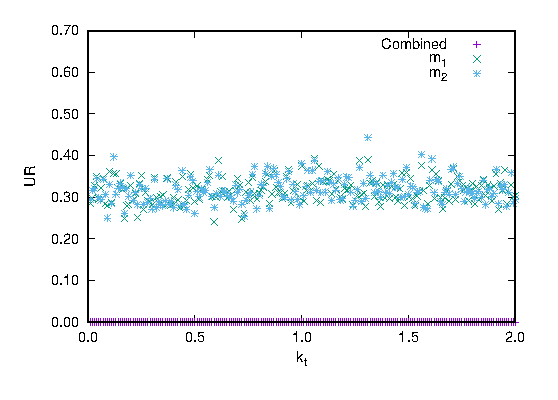
\includegraphics[keepaspectratio,scale=0.8]{case1_mean_hikaku.eps}
      \subcaption{期待値}
      \label{fig:hikaku1}
    \end{minipage} &
    \begin{minipage}[t]{0.45\hsize}
      \centering
      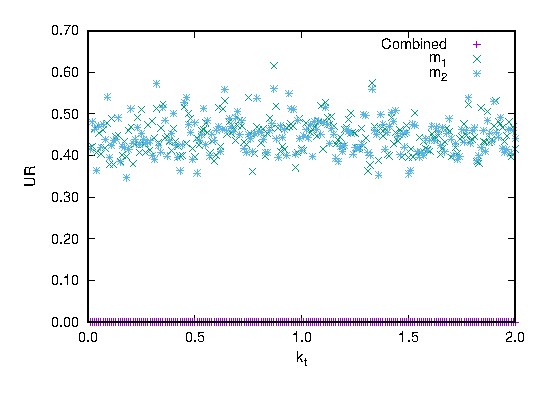
\includegraphics[keepaspectratio,scale=0.8]{case1_deviation_hikaku.eps}
      \subcaption{標準偏差}
      \label{fig:hikaku2}
    \end{minipage} 
  \end{tabular}
  \caption{単一パラメータと複数パラメータ組み合わせの比較}
  \label{fig:hikaku}
\end{figure}

このように、無次元化を施した場合であっても
複数パラメータの組み合わせは単一パラメータのみを用いた場合と比較して誤差の低減に効果的な手段であると言える。

続いて、ケース1を用いて重み$a_i$を算出したものを図\ref{fig:weight}に示す。

\begin{figure}[H]
  \centering
  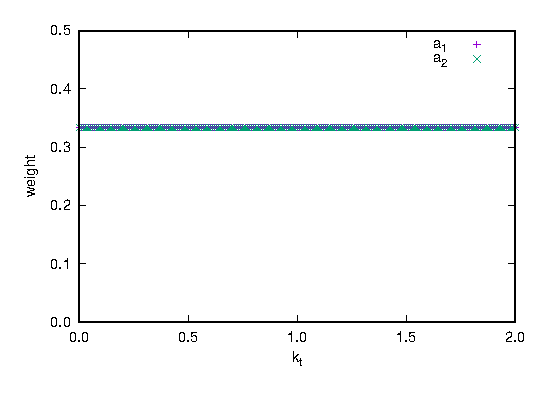
\includegraphics[keepaspectratio,scale=1.0]{case1_weight.eps}
  \caption{重み}
  \label{fig:weight}
\end{figure}

ここで、重み$a_i$の厳密解は以下の式(\ref{eq:weight})の、$\frac{\partial p_{m}}{\partial \sigma_i} = S_{m_i}$についての連立方程式を解くことによって計算することができる。
\begin{equation}
  \frac{\partial p_{m}}{\partial \sigma} = \left(p_{m_1}^{a_1} p_{m_2}^{a_2}\right) \left(\frac{a_1}{p_{m_1}}\frac{\partial p_{m_1}}{\partial \sigma} + \frac{a_2}{p_{m_2}}\frac{\partial p_{m_2}}{\partial \sigma} \right)
  \label{eq:weight}
\end{equation}
式(\ref{eq:weight})を用いた厳密解は$a_1 = a_2 = 1/3$となり、これは図\ref{fig:weight}と一致する。

一方で、式(\ref{eq2.22})の$\bm{\Sigma}_{m}$を既知の値を用いて計算した場合、結果は図\ref{fig:rig}、重みは図\ref{fig:weight2}となる。

\begin{figure}[H]
  \begin{tabular}{cc}
    \begin{minipage}[t]{0.45\hsize}
      \centering
      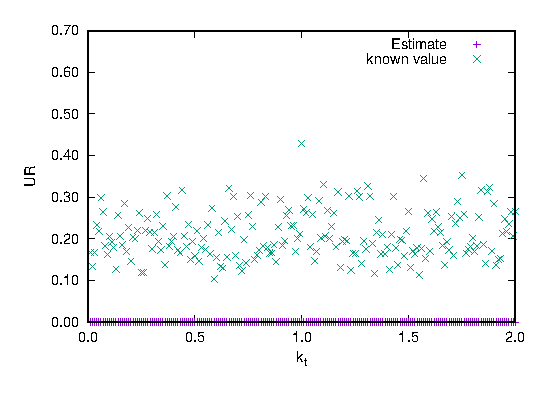
\includegraphics[keepaspectratio,scale=0.8]{case1_mean_rig.eps}
      \subcaption{期待値}
      \label{fig:mean_rig}
    \end{minipage} &
    \begin{minipage}[t]{0.45\hsize}
      \centering
      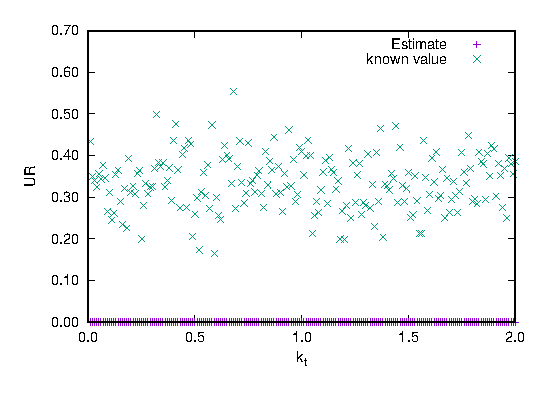
\includegraphics[keepaspectratio,scale=0.8]{case1_deviation_rig.eps}
      \subcaption{標準偏差}
      \label{fig:deviation_rig}
    \end{minipage} 
  \end{tabular}
  \caption{ケース1}
  \label{fig:rig}
\end{figure}

\begin{figure}[H]
  \centering
  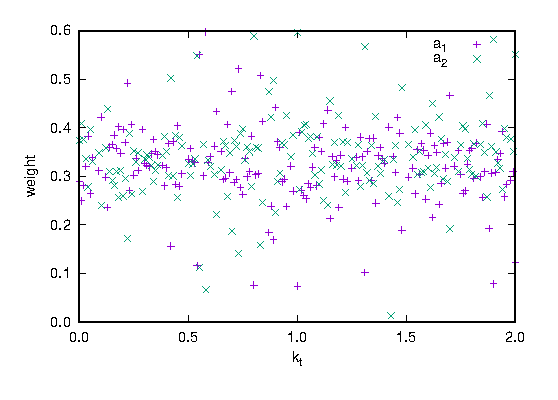
\includegraphics[keepaspectratio,scale=1.0]{case1_weight2.eps}
  \caption{既知の値を用いて求めた重み}
  \label{fig:weight2}
\end{figure}

既知の値を用いた場合ではURが大きくなり、重みは厳密解と一致しないことが分かる。
このように、標本から求めた統計量を用いることで推定精度を向上させることが可能である。

\section{結果、考察}
得られた結果を図\ref{fig:19}から図\ref{fig:43}までに示す。

\begin{figure}[H]
  \begin{tabular}{cc}
    \begin{minipage}[t]{0.45\hsize}
      \centering
      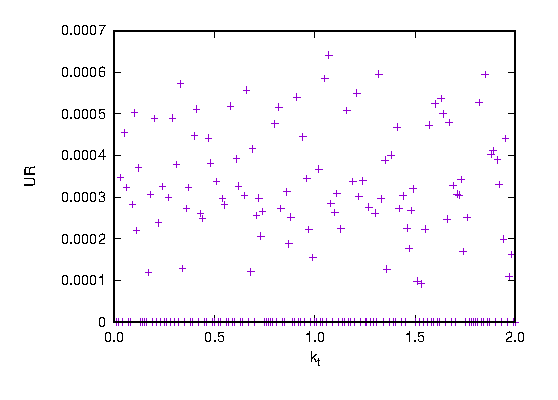
\includegraphics[keepaspectratio,scale=0.8]{case1_mean.eps}
      \subcaption{期待値}
      \label{fig:17}
    \end{minipage} &
    \begin{minipage}[t]{0.45\hsize}
      \centering
      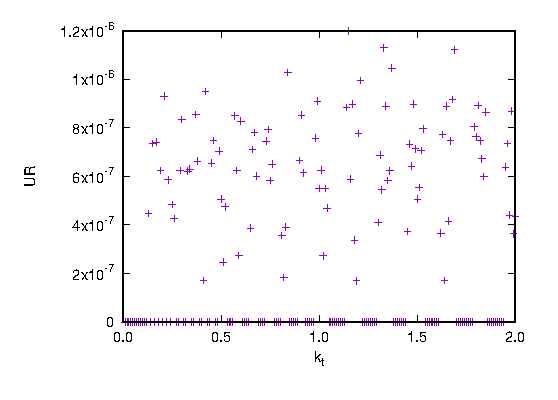
\includegraphics[keepaspectratio,scale=0.8]{case1_deviation.eps}
      \subcaption{標準偏差}
      \label{fig:18}
    \end{minipage} 
  \end{tabular}
  \caption{ケース1}
  \label{fig:19}
\end{figure}

\begin{figure}[H]
  \begin{tabular}{cc}
    \begin{minipage}[t]{0.45\hsize}
      \centering
      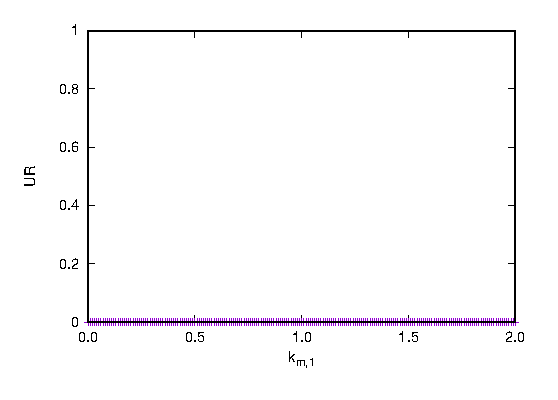
\includegraphics[keepaspectratio,scale=0.8]{case2_mean.eps}
      \subcaption{期待値}
      \label{fig:20}
    \end{minipage} &
    \begin{minipage}[t]{0.45\hsize}
      \centering
      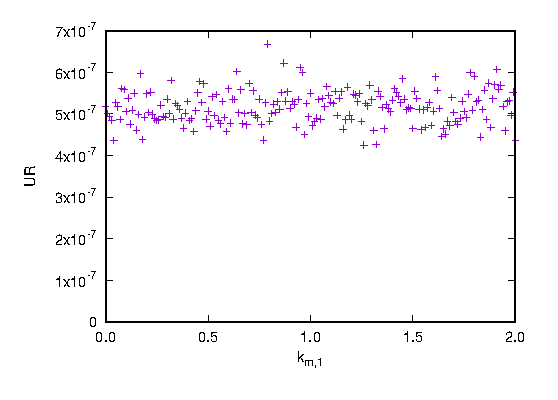
\includegraphics[keepaspectratio,scale=0.8]{case2_deviation.eps}
      \subcaption{標準偏差}
      \label{fig:21}
    \end{minipage} 
  \end{tabular}
  \caption{ケース2}
  \label{fig:22}
\end{figure}

\begin{figure}[H]
  \begin{tabular}{cc}
    \begin{minipage}[t]{0.45\hsize}
      \centering
      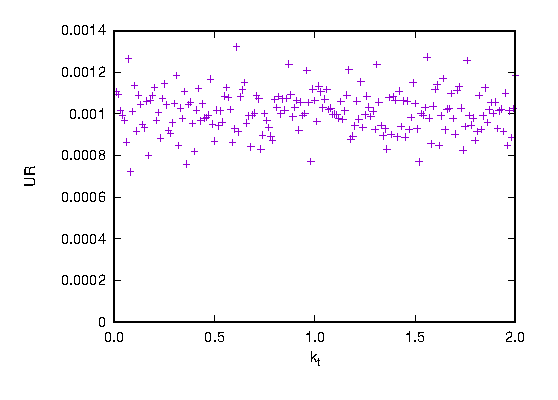
\includegraphics[keepaspectratio,scale=0.8]{case3_mean.eps}
      \subcaption{期待値}
      \label{fig:23}
    \end{minipage} &
    \begin{minipage}[t]{0.45\hsize}
      \centering
      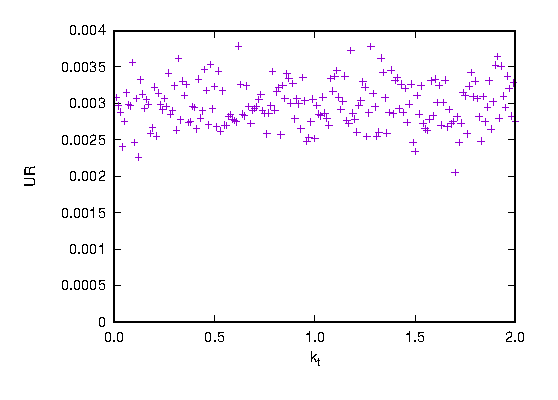
\includegraphics[keepaspectratio,scale=0.8]{case3_deviation.eps}
      \subcaption{標準偏差}
      \label{fig:24}
    \end{minipage} 
  \end{tabular}
  \caption{ケース3}
  \label{fig:25}
\end{figure}

\begin{figure}[H]
  \begin{tabular}{cc}
    \begin{minipage}[t]{0.45\hsize}
      \centering
      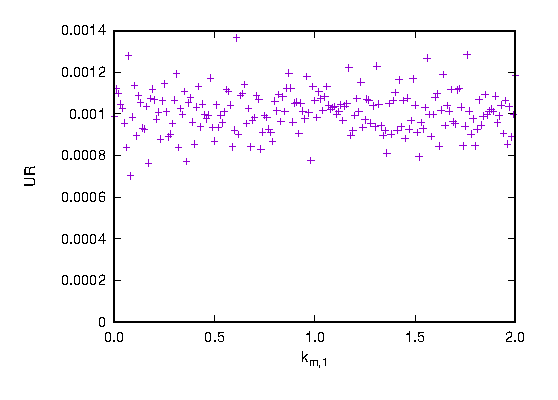
\includegraphics[keepaspectratio,scale=0.8]{case4_mean.eps}
      \subcaption{期待値}
      \label{fig:26}
    \end{minipage} &
    \begin{minipage}[t]{0.45\hsize}
      \centering
      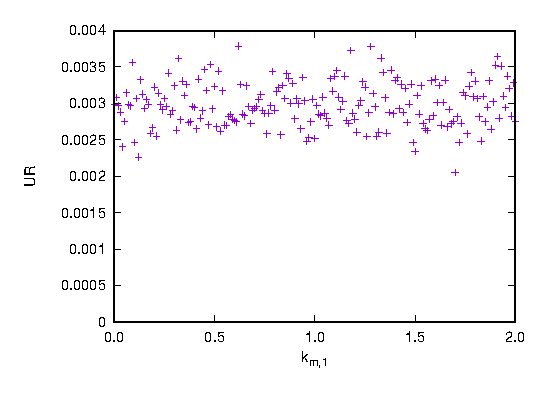
\includegraphics[keepaspectratio,scale=0.8]{case4_deviation.eps}
      \subcaption{標準偏差}
      \label{fig:27}
    \end{minipage} 
  \end{tabular}
  \caption{ケース4}
  \label{fig:28}
\end{figure}

\begin{figure}[H]
  \begin{tabular}{cc}
    \begin{minipage}[t]{0.45\hsize}
      \centering
      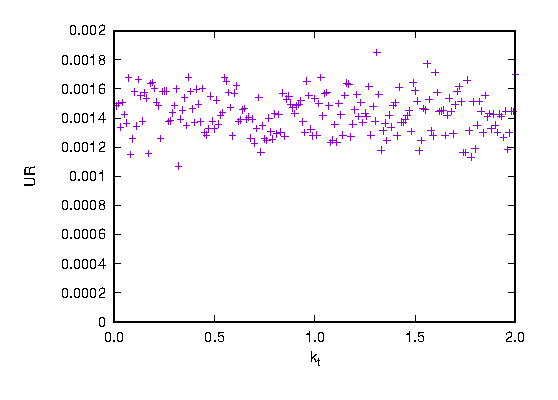
\includegraphics[keepaspectratio,scale=0.8]{case5_mean.eps}
      \subcaption{期待値}
      \label{fig:29}
    \end{minipage} &
    \begin{minipage}[t]{0.45\hsize}
      \centering
      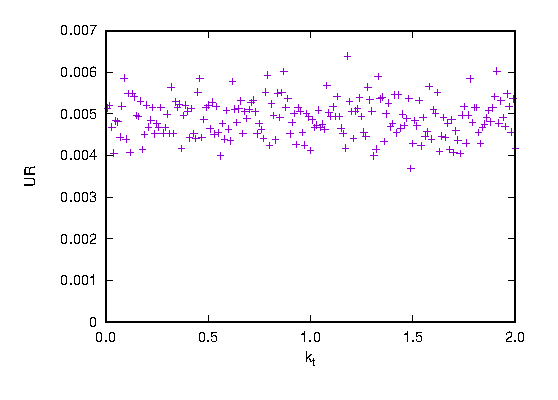
\includegraphics[keepaspectratio,scale=0.8]{case5_deviation.eps}
      \subcaption{標準偏差}
      \label{fig:30}
    \end{minipage} 
  \end{tabular}
  \caption{ケース5}
  \label{fig:31}
\end{figure}

\begin{figure}[H]
  \begin{tabular}{cc}
    \begin{minipage}[t]{0.45\hsize}
      \centering
      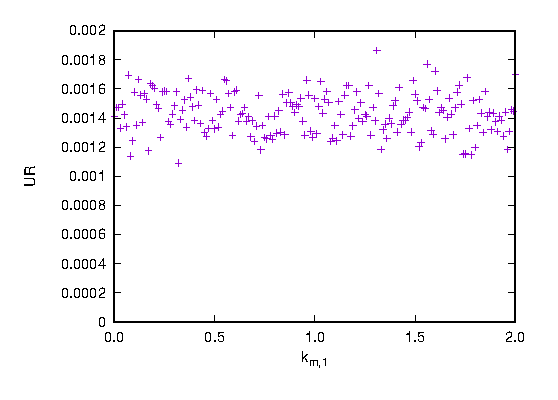
\includegraphics[keepaspectratio,scale=0.8]{case6_mean.eps}
      \subcaption{期待値}
      \label{fig:32}
    \end{minipage} &
    \begin{minipage}[t]{0.45\hsize}
      \centering
      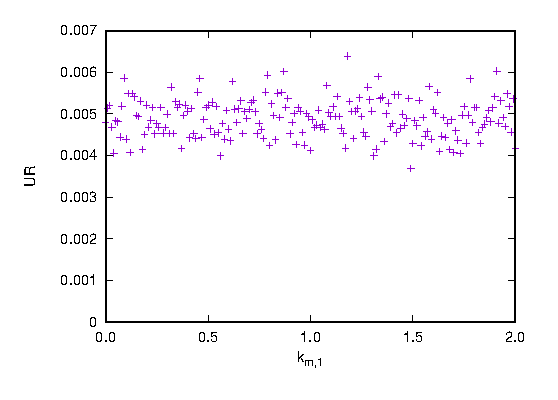
\includegraphics[keepaspectratio,scale=0.8]{case6_deviation.eps}
      \subcaption{標準偏差}
      \label{fig:33}
    \end{minipage} 
  \end{tabular}
  \caption{ケース6}
  \label{fig:34}
\end{figure}

\begin{figure}[H]
  \begin{tabular}{cc}
    \begin{minipage}[t]{0.45\hsize}
      \centering
      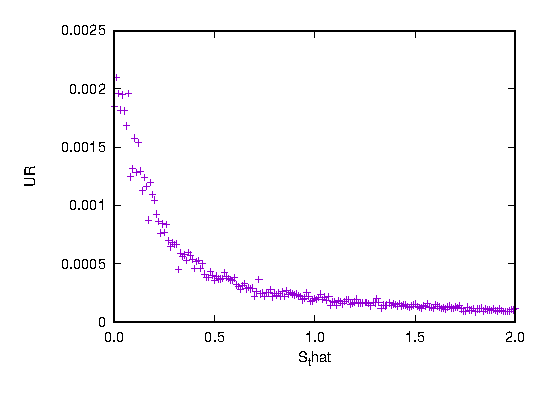
\includegraphics[keepaspectratio,scale=0.8]{case7_mean.eps}
      \subcaption{期待値}
      \label{fig:35}
    \end{minipage} &
    \begin{minipage}[t]{0.45\hsize}
      \centering
      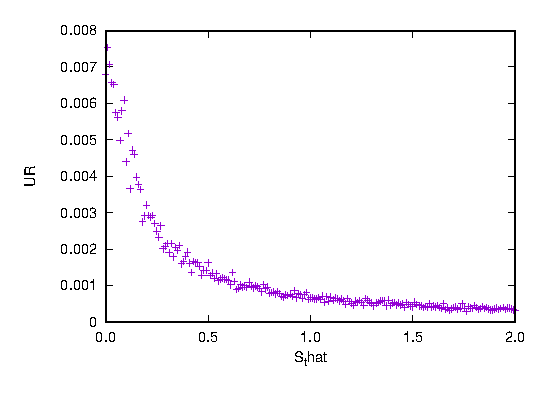
\includegraphics[keepaspectratio,scale=0.8]{case7_deviation.eps}
      \subcaption{標準偏差}
      \label{fig:36}
    \end{minipage} 
  \end{tabular}
  \caption{ケース7}
  \label{fig:37}
\end{figure}

\begin{figure}[H]
  \begin{tabular}{cc}
    \begin{minipage}[t]{0.45\hsize}
      \centering
      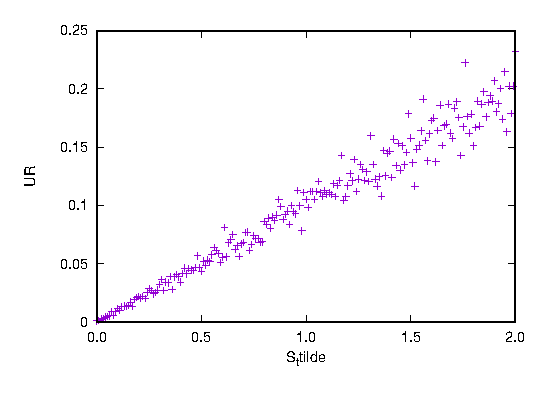
\includegraphics[keepaspectratio,scale=0.8]{case8_mean.eps}
      \subcaption{期待値}
      \label{fig:38}
    \end{minipage} &
    \begin{minipage}[t]{0.45\hsize}
      \centering
      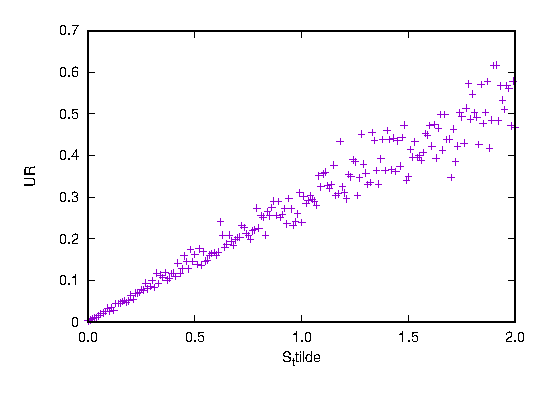
\includegraphics[keepaspectratio,scale=0.8]{case8_deviation.eps}
      \subcaption{標準偏差}
      \label{fig:39}
    \end{minipage} 
  \end{tabular}
  \caption{ケース8}
  \label{fig:40}
\end{figure}

\begin{figure}[H]
  \begin{tabular}{cc}
    \begin{minipage}[t]{0.45\hsize}
      \centering
      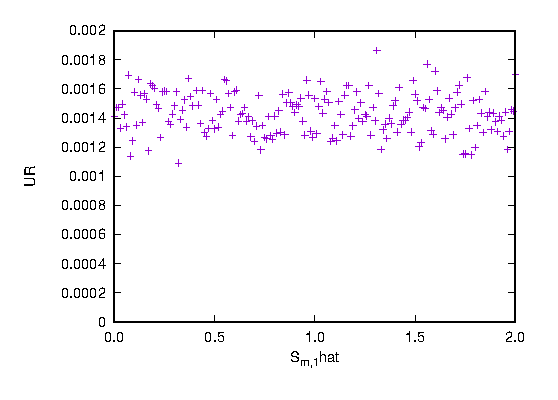
\includegraphics[keepaspectratio,scale=0.8]{case9_mean.eps}
      \subcaption{期待値}
      \label{fig:41}
    \end{minipage} &
    \begin{minipage}[t]{0.45\hsize}
      \centering
      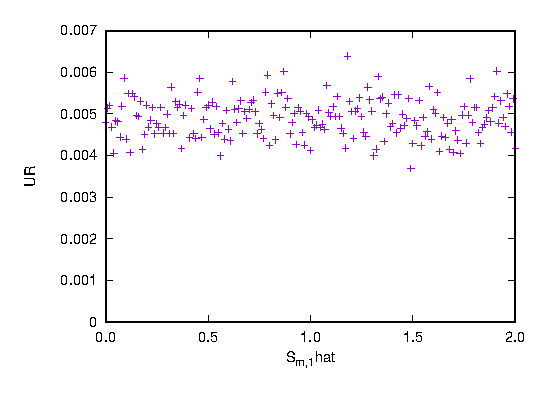
\includegraphics[keepaspectratio,scale=0.8]{case9_deviation.eps}
      \subcaption{標準偏差}
      \label{fig:42}
    \end{minipage} 
  \end{tabular}
  \caption{ケース9}
  \label{fig:43}
\end{figure}

以上の結果から、URに対して影響を及ぼすパラメータが$\hat{S_t}$および$\tilde{S_t}$であることがわかる。
さらに、ケース7とケース8の結果から、URは$\tilde{S_t}/\hat{S_t}$に比例して大きくなると考えられる。
これは、対象パラメータにおける$\tilde{S_t}$の影響、すなわち模擬パラメータには存在しない二次の項の影響が大きくなることで、
対象パラメータと模擬パラメータの相関が小さくなるためである。

その他の影響は除かれていることから、無次元化は有効な手段だといえる。

以上の結果から、無次元化と複数パラメータによる仮想的なパラメータを組み合わせることで、より効率的に
不確かさを推定することが可能であることが明らかとなった。
\newpage

\chapter{燃料ピンセル体系への適用}
\section{概要}
簡易問題では、前述の手法が有効な手段であることが示された。そのため、これを実際の問題に適用し、その有用性について更なる検証を行った。

本検討ではまず、燃料ピンセル体系での燃焼度ごとの無限増倍率$k_{inf}$の標準偏差の不確かさを、核種数密度を模擬パラメータとして用いることで推定した。
詳細な条件を以下に示す。

\begin{itemize}
  \item 計算対象…燃料ピンセル体系
  \item 燃料…4.1wt\% \space UO2燃料
  \item 対象パラメータ…21燃焼度($0,0.1,1.0,2.5,5.0,~,45.0 \mathrm{GWD/t}$)における$k_{inf}$
  \item 模擬パラメータ…\begin{itemize}
    \item 燃焼度5$\mathrm{GWD/t}$におけるPu-239核種数密度の核データに対するに対する一次近似
    \item 燃焼度40$\mathrm{GWD/t}$におけるPu-242核種数密度の核データに対するに対する一次近似
  \end{itemize}
\end{itemize}

なお、模擬パラメータの選出基準については、文献\cite{Harada}より、$k_{inf}$に対する寄与が大きい2種類の核種数密度を選択している。

分散の推定は10000個のサンプルを用いたCV法で行い、推定した分散の標準誤差は後述するブートストラップ法で求めた。

\section{ブートストラップ法}
ブートストラップ法とは、あらかじめサンプリングされた標本から、改めてサンプリングを行い、リサンプリングされた確率変数についての統計量を求め、複数回行ったリサンプリングの統計量について、
さらに統計的に評価をすることで、標本の統計量を評価する手法である\cite{efron1986bootstrap}\cite{endo2015confidence}。

この手法では、あらかじめ求められた標本を対象としているため、繰り返し計算をする場合に都度対象のパラメータを計算する必要がない。これは、パラメータを求める際に多大な計算コストがかかる
燃料集合体体系などで非常に有効な手法であるといえる。

本検討では、10000個の標本から10000のリサンプリングを行い、リサンプリングされた標本から統計量を推定した。

\section{結果・考察}
まず初めに、20$\mathrm{GWD/t}$における、各手法を用いて推定された標準偏差、および標準誤差を図\ref{fig:20g}に示す。
\begin{figure}[H]
  \centering
  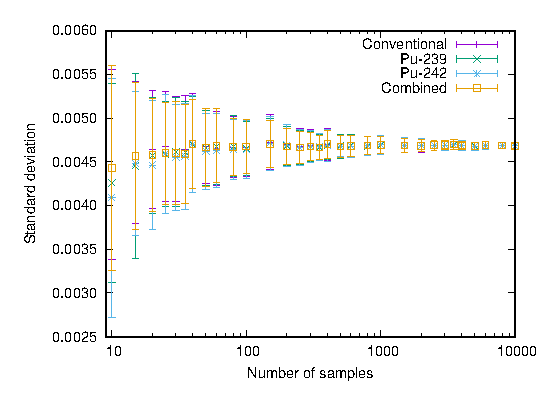
\includegraphics{std.eps}
  \caption{20$\mathrm{GWD/t}$における標準偏差、および標準誤差}
  \label{fig:20g}
\end{figure}
このように、いずれの方法を用いた場合であっても、推定される結果に偏りは発生していない。

続いて、URを求めた結果を図\ref{fig:2mockup}に示す。

\begin{figure}[H]
  \centering
  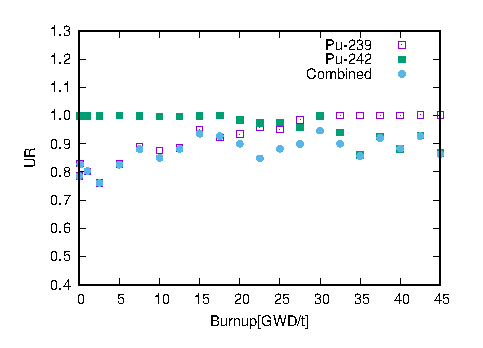
\includegraphics{2mockup_data.eps}
  \caption{核種数密度を用いた$k_{inf}$の不確かさ推定}
  \label{fig:2mockup}
\end{figure}
このように、模擬パラメータを単一で用いた場合には特定の燃焼度範囲のみ誤差の低減がなされているのに対し、組み合わせることで全体を通して誤差を低減していることが確認できる。
しかし、複数パラメータを組み合わせた場合であっても、URの数値としては良い結果を得られなかった。

この原因として、対象パラメータ$k_{inf}$に対して模擬パラメータが核種数密度と、用いたデータがそれぞれ異なる種類のものであったため、
元々のパラメータ間の相関が小さくなってしまったことが挙げられる。

図\ref{fig:2mockup_corr}に模擬パラメータと対象のパラメータの相関を示すが、それぞれ単一の模擬パラメータと対象パラメータの相関は最大でも0.7程度であり、これらを組み合わせた場合であってもその最大値は大きく変化しない。
既往研究により、相関が0.8未満では誤差の低減が十分に行われないことが明らかとなっているため、今回の検証では十分な誤差の低減が為されなかったと言える。
\begin{figure}[H]
  \centering
  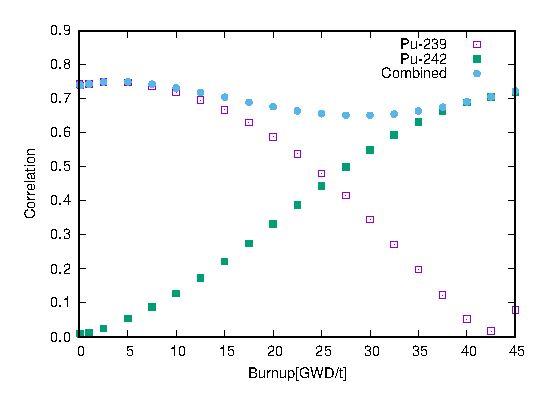
\includegraphics{2mockup_corr.eps}
  \caption{対象パラメータと模擬パラメータの相関}
  \label{fig:2mockup_corr}
\end{figure}

次に示した図\ref{fig:2mockup_imp}では、模擬パラメータを
\begin{itemize}
  \item 燃焼度5$\mathrm{GWD/t}$における$k_{inf}$
  \item 燃焼度40$\mathrm{GWD/t}$における$k_{inf}$
\end{itemize}
としている。なお、これらの模擬パラメータは核データに対する線形近似ではない。

\begin{figure}[H]
  \centering
  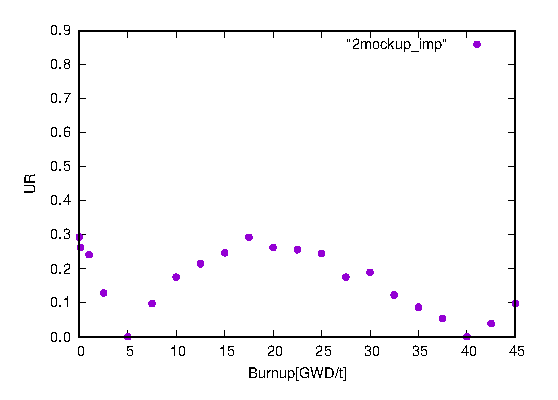
\includegraphics{2mockup_imp.eps}
  \caption{$k_{inf}$を用いた$k_{inf}$の不確かさ推定}
  \label{fig:2mockup_imp}
\end{figure}
この図からわかる通り、使用したパラメータの数は図\ref{fig:2mockup}と同様であるにもかかわらず、URの値は改善されている。
ここから、模擬パラメータとして使用するデータについても、例えば燃料集合体体系における$k_{inf}$を対象とした場合、燃料ピンセル体系における$k_{inf}$を用いるなど、
ある程度相関が保証されたものを用いるべきだと言える。

最後に、模擬パラメータを初期の2つに加えて
\begin{itemize}
  \item 燃焼度40$\mathrm{GWD/t}$におけるPu-239核種数密度の核データに対する一次近似
  \item 燃焼度20$\mathrm{GWD/t}$におけるPu-240の核種数密度核データに対する一次近似
  \item 燃焼度10$\mathrm{GWD/t}$におけるPu-242の核種数密度核データに対する一次近似
  \item 燃焼度30$\mathrm{GWD/t}$におけるPu-242の核種数密度核データに対する一次近似
\end{itemize}
を追加し、計6つのデータを模擬パラメータとして、同様に不確かさの推定を行った。追加された模擬パラメータについても、文献\cite{Harada}より、$k_{inf}$への影響の大きい核種数密度を選出している。

こちらは、5296個のサンプルから5000個をリサンプリングする点を除いて、手順は模擬パラメータが2つの場合と同様である。

その結果を図\ref{fig:6mockup}に示す。
\begin{figure}[H]
  \centering
  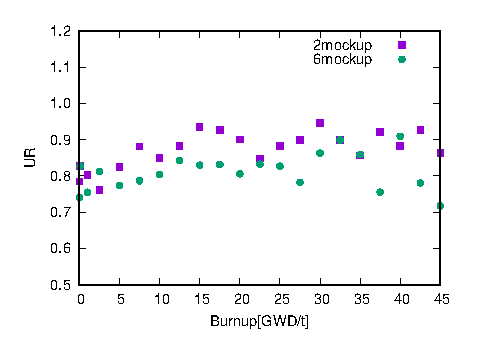
\includegraphics{6mockup.eps}
  \caption{模擬パラメータを6個用いた$k_{inf}$の不確かさ推定}
  \label{fig:6mockup}
\end{figure}

模擬パラメータを二つ用いた場合と比較し、わずかであるが値が改善してる。このように、模擬パラメータを増やすことでも、不確かさの低減を効率的に行うことができると考えられる。
\newpage

\chapter{まとめ}
本研究では、CV-S法の改善手法として検討されてきた2つの手法について、それらを組み合わせて用いた場合の有効性について検討した。
その結果、無次元化による対象パラメータと模擬パラメータの統計量の影響の排除、
および複数の模擬パラメータの組み合わせによるさらなる不確かさ推定の精度向上を、これらを組み合わせることによっても再現することが可能であることが示された。

また、実際の問題に適用した場合、初期の検討では数値として十分な結果を得ることができなかった。
しかし、その後の追加の検討により、ある程度の相関が保証されているパラメータを用いることで、
計算結果を向上させるに至った。加えて、模擬パラメータを増加させることでも、
計算結果を改善できることが示された。

以上の結果を以て、本研究により検討された手法は実際の問題に適用が可能であると考える。よって、今後の研究ではこの手法を用いて
不確かさの推定を行う計算コードを開発していく。

\newpage

\bibliography{graduation} %hoge.bibから拡張子を外した名前
\bibliographystyle{junsrt} %参考文献出力スタイル

\chapter*{謝辞}
本研究を進めるにあたり、千葉豪准教授にはさまざまなご指摘、ご指導を賜りましたこと、深く感謝しております。
また、普段からお世話になりました先輩方、同期の皆様にも感謝いたします。

\end{document}